\documentclass[conference]{IEEEtran}
\IEEEoverridecommandlockouts

\usepackage{cite}
\usepackage{amsmath,amssymb,amsfonts}
\usepackage{algorithmic}
\usepackage{algorithm}
\usepackage{graphicx}
\usepackage{textcomp}
\usepackage{xcolor}
\usepackage{booktabs}
\usepackage{tikz}
\usepackage{url}
\usepackage{multirow}
\usepackage{siunitx}
\usetikzlibrary{shapes.geometric, arrows.meta, positioning, fit, backgrounds, calc}
\newcommand{\cmark}{\checkmark}

\def\BibTeX{{\rm B\kern-.05em{\sc i\kern-.025em b}\kern-.08em
    T\kern-.1667em\lower.7ex\hbox{E}\kern-.125emX}}

\begin{document}

\title{Robust Chess Opening Repertoire Optimization via\\
Co-Evolutionary Genetic Algorithms and a Closure Constraint}

\author{\IEEEauthorblockN{Minhaj ul Hassan}
\IEEEauthorblockA{\textit{Department of Computer Science} \\
\textit{Habib University}\\
Karachi, Pakistan \\
mu08984@st.habib.edu.pk}
\and
\IEEEauthorblockN{Zainab Zahid}
\IEEEauthorblockA{\textit{Department of Computer Science} \\
\textit{Habib University}\\
Karachi, Pakistan \\
zz08969@st.habib.edu.pk}
\and
\IEEEauthorblockN{Hazeera Muhammad Hashim}
\IEEEauthorblockA{\textit{Department of Computer Science} \\
\textit{Habib University}\\
Karachi, Pakistan \\
hm09247@st.habib.edu.pk}
}

\maketitle

% -------------------------------------------------------------------------
\begin{abstract}
Building a chess opening repertoire means pre-memorizing a compact set of
moves that hold up against a variety of opponents. Current tools handle this
greedily---selecting moves by frequency or win rate---without jointly
optimizing for robustness across skill levels or ensuring the repertoire
covers all dangerous opponent replies. We formalize the task as constructing
a budget-constrained subgraph of a chess position graph built from Lichess
rapid and classical games, and introduce a \emph{closure rule}: at every
position where the opponent moves, all replies played in at least 15\% of
observed games must be covered. A CVaR-weighted fitness objective across
three rating bands (1000--1399, 1400--1799, 1800--2199) rewards both mean
performance and robustness against the worst-case opponent skill level. We
optimize this using a co-evolutionary genetic algorithm ({\scshape Coevolve}),
which co-adapts a population of opponent strategies alongside the repertoire
population, and compare it against a static GA ({\scshape Static}), a greedy
hillclimber, random search, and a most-played heuristic. Across 30 independent
seeds and two budget conditions ($B \in \{10, 25\}$ committed moves per color),
the closure rule is the dominant factor: it yields a consistent +2.3
percentage-point improvement in held-out expected score with perfect effect
size ($A_{12} = 1.0$, $p < 7.5 \times 10^{-9}$, Wilcoxon signed-rank with
Holm correction), and every single seed performs better with the rule than
without it. Co-evolution, by contrast, offers no statistically significant
benefit over the static GA ($p = 1.0$, $A_{12} = 0.45$) at 35$\times$ the
computational cost. A greedy hillclimber matches GA-quality solutions at a
fraction of the runtime, suggesting the closure-constrained fitness landscape
responds well to local search.
\end{abstract}

\begin{IEEEkeywords}
chess, opening repertoire, genetic algorithm, co-evolutionary computation,
CVaR, robust optimization, Lichess
\end{IEEEkeywords}


% =========================================================================
\section{Introduction}

Chess opening preparation is a central part of competitive play at every
level. A player needs to select a compact \emph{repertoire}---a set of
preferred responses for both colors---that holds up against the range of
opponents they are likely to face. This is an optimization problem under
constraints: the player has limited memorization capacity, must anticipate
a distribution of opponent responses, and ideally should perform well
across skill levels rather than against just one type of player.

Current computer-aided tools---including Lichess Opening Explorer
\cite{lichess}, SCID, and ChessBase---let players browse game databases
and pick moves by frequency or win rate. These tools are useful but
limited: they do not jointly optimize a global repertoire objective, they
do not ensure coverage of dangerous opponent replies, and they do not
account for how opponent behavior shifts with skill level.

What makes this problem genuinely hard is the scale of the search space.
A database of real games exposes hundreds of distinct positions, and
combining them into a coherent repertoire---one that covers all critical
opponent replies without wasting the memorization budget on marginal
lines---involves a combinatorial search that is neither convex nor
continuous. Picking lines purely by win rate ignores coverage gaps and
the fact that different skill levels play very differently. Moreover, what
makes a repertoire ``good'' is not fixed: lines that work against a
positional player can fail against an aggressive one, and a repertoire
tuned for average performance can hide systematic weaknesses that overall
statistics simply obscure.

This paper presents a fully automated system for repertoire optimization.
Given millions of Lichess games organized by rating band, the system builds
a position graph, computes per-band move statistics, and uses a genetic
algorithm to find a compact opening repertoire. A genetic algorithm is
particularly well suited here: the repertoire space is discrete and
non-convex, changing one committed move can cascade through the tree, and
gradient methods do not apply to move choices. A population of candidates
explores the space in parallel; a co-evolving opponent population provides
adaptive adversarial pressure at no extra architectural cost. The central
design choice is the \textbf{closure rule}: at every position where the
opponent moves, all replies played in at least $\theta = 0.15$ of observed
games must be covered. This forces the system to handle the most likely
opponent continuations rather than cherry-picking only the best-case lines.

We propose two GA variants. {\scshape Static} evaluates repertoires against
a fixed, uniform mix of all three rating bands. {\scshape Coevolve} goes
further, maintaining a co-evolving population of opponent strategies that
adapts to challenge the current repertoire population, guided by both
performance and novelty. We compare both variants against a greedy
hillclimber, random search, and a most-played heuristic at a matched
evaluation budget.

\textbf{Contributions:}
\begin{enumerate}
  \item A formal repertoire model defined as a budget-constrained subgraph
        of the chess position graph, with a closure rule and a CVaR-robust
        fitness function that rewards robustness across opponent skill levels.
  \item A co-evolutionary GA with adaptive opponent modeling, novelty-driven
        opponent fitness, and a Hall of Fame of informative opponents.
  \item Controlled evaluation over 30 seeds and two budget conditions, using
        Wilcoxon signed-rank tests and Vargha-Delaney $A_{12}$ effect sizes.
\end{enumerate}

\textbf{Main findings:} The closure rule is the decisive contribution
(+2.3~pp, $A_{12} = 1.0$). Co-evolution adds no measurable benefit over
the static GA ($p = 1.0$, $A_{12} = 0.45$) at 35$\times$ the computational
cost. The greedy hillclimber matches both GA variants and offers the best
accuracy-to-cost tradeoff.


% =========================================================================
\section{Related Work}

\textbf{Chess databases and opening book tools.}
Walczak~\cite{walczak1996} showed that adapting an opening book to model
opponent style produces measurable improvements---an early indication that
opponent-awareness matters in opening preparation. Fogel~\cite{fogel2004}
applied neuroevolution to train a self-learning chess evaluation function,
establishing evolutionary computation as a viable approach to chess-specific
optimization. More recently, Marzo and Servedio~\cite{marzo2023} analyzed
large-scale Lichess data and found statistically significant differences in
move preferences across rating bands, which directly motivates our per-band
fitness formulation.

\textbf{Co-evolutionary algorithms.}
Co-evolution refers to simultaneously evolving two interacting populations so
that each drives improvement in the other. Hillis~\cite{hillis1990} demonstrated
this in sorting networks, showing that co-evolving ``parasite'' programs
prevents premature convergence. Rosin and Belew~\cite{rosin1997} formalized
competitive co-evolution and introduced the Competitive Fitness Archive to
handle cycling and intransitivity; our Hall of Fame mechanism is directly
inspired by that idea. Ramos et al.~\cite{ramos2016} applied co-evolutionary
methods to chess program development, providing a close precedent for the
approach we take here.

\textbf{Novelty and diversity.}
Lehman and Stanley~\cite{lehman2011} showed that optimizing for behavioral
novelty---rather than a fixed objective---can outperform conventional
goal-directed search. We incorporate novelty as a secondary component of
opponent fitness to prevent the opponent population from collapsing to a
single adversarial mixture strategy.

\textbf{Robust and risk-aware optimization.}
CVaR (Conditional Value at Risk) is a standard measure for penalizing
worst-case outcomes rather than just averaging over them
\cite{rockafellar2000}. We apply it across rating bands: the fitness
function balances mean score with performance on the worst-performing
band, which incentivizes robustness across skill levels rather than
specialization toward one type of opponent.


% =========================================================================
\section{Problem Formulation}

\subsection{Position Graph}

The foundation of our model is a directed graph where each node is a chess
position and each edge is a legal move. Formally, let
$\mathcal{G} = (\mathcal{V}, \mathcal{E})$ be a directed acyclic graph
where each node $v \in \mathcal{V}$ is a canonical chess position represented
as a truncated FEN string (piece placement, active color, castling rights, and
en passant field only; halfmove and fullmove clocks are stripped to collapse
transpositions). Each directed edge $(v, v') \in \mathcal{E}$ represents a
legal move from $v$ to $v'$. Every node $v$ carries a turn indicator
$\tau(v) \in \{\text{white}, \text{black}\}$ and a ply depth
$d(v) \in \{0, 1, \ldots, D_{\max}\}$ with $D_{\max} = 10$.
For each rating band $b \in \mathcal{B} = \{1000\text{-}1399,\,
1400\text{-}1799,\, 1800\text{-}2199\}$, each edge $(v, v')$ stores a
play count $N_b(v, v')$ and outcome statistics (white wins, draws, losses)
from the Lichess game database.

\subsection{Per-Band Move Policies}

Each rating band has its own characteristic move preferences. We model
this as a smoothed probability distribution over moves at each position,
blending band-specific counts with the aggregate (all-ratings) distribution
to handle sparse positions. For band $b$ and position $v$, the policy
$p_b(m \mid v)$ gives the probability that a player in band $b$ plays
move $m$:
\begin{equation}
  p_b(m \mid v) =
  \frac{N_b(v, m) + \alpha\, p_{\mathrm{agg}}(m \mid v)}
       {\displaystyle\sum_{m'} N_b(v, m') + \alpha},
  \label{eq:policy}
\end{equation}
where $p_{\mathrm{agg}}(m \mid v) = N_{\mathrm{agg}}(v,m) /
\sum_{m'} N_{\mathrm{agg}}(v, m')$ is the aggregate (all-rating) move
probability and $\alpha = 5.0$ provides additive smoothing toward the
aggregate distribution.

\subsection{Position Evaluation Cache}

To score positions without simulating full games, we estimate the expected
White win rate at each position using an empirical-Bayes shrinkage estimator:
observed outcomes are blended with a global prior to handle positions with
few games. Concretely, the estimated White-perspective win score at position
$v$ in band $b$ is:
\begin{equation}
  \hat{v}_b(v) =
  \frac{N_b(v) \cdot r_b(v) + \tau\, \mu_0}{N_b(v) + \tau},
  \label{eq:eval}
\end{equation}
where $r_b(v) = (\text{wins}_b + 0.5 \cdot \text{draws}_b) / N_b(v)$
is the raw White win rate, $\tau = 20$ is the regularization strength,
and $\mu_0$ is the global prior mean (average of $\hat{v}$ over all
positions at depth $\leq D_{\max}$ in the training set). For positions
with $N_b(v) = 0$, we use $\hat{v}_b(v) = \mu_0$.

\subsection{Repertoire and Closure Constraint}

A repertoire is not simply a list of moves---it is a strategy tree.
At positions where it is our turn, we commit to a single move. At
positions where the opponent moves, we must be prepared for every reply
they are likely to make. We formalize this as follows.

A \textbf{repertoire} for color $c \in \{\text{white}, \text{black}\}$
with budget $B$ is a pair $\mathcal{R} = (\phi, \mathcal{S})$ where
$\phi : \mathcal{V}_c \to \mathcal{E}$ is a partial function mapping
our-color positions to committed moves (with $|\phi| \leq B$), and
$\mathcal{S} \subseteq \mathcal{V}$ is the \emph{reached set}: all
positions reachable by following $\phi$ at our-turn nodes and following
all covered opponent moves at opponent-turn nodes.

The \textbf{closure rule} enforces coverage completeness. At every
opponent-turn position $v \in \mathcal{S}$, any move the opponent plays
in at least $\theta = 0.15$ of observed games must lead to another
position in the reached set:
\begin{equation}
  p_{\mathrm{agg}}(m \mid v) \geq \theta
  \;\Rightarrow\;
  \mathrm{ch}(v, m) \in \mathcal{S},
  \qquad \forall\, v \in \mathcal{S},\; \tau(v) \neq c.
  \label{eq:closure}
\end{equation}
In plain terms: the repertoire cannot ignore a common opponent reply just
because it is inconvenient. Operationally, whenever a committed move
expands the reached set, a breadth-first pass adds all opponent replies
above the threshold recursively.

\subsection{Recursive Evaluation}

Given a repertoire, we compute its expected score against a rating band
by walking the strategy tree. The recursion $W_b(v, \mathcal{R})$ is
defined as follows, where $\mathrm{ch}(v,m)$ denotes the child position
after move $m$:
\begin{equation}
W_b(v, \mathcal{R}) =
\begin{cases}
  W_b\!\bigl(\mathrm{ch}(v, \phi(v)),\, \mathcal{R}\bigr)
      & \tau(v)=c,\;\phi(v)\text{ defined}\\[4pt]
  \hat{v}_b(v)
      & \tau(v)=c,\;\text{(leaf)}\\[4pt]
  \sum_{m} p_b(m \mid v)\, W_b\!\bigl(\mathrm{ch}(v,m), \mathcal{R}\bigr)
      & \tau(v)\neq c
\end{cases}
\label{eq:walk}
\end{equation}
The three cases correspond to: follow our committed move, fall back to
the cached score at a leaf, or average over opponent replies weighted by
their band probability. Positions not in $\mathcal{S}$ are treated as
leaves with score $\hat{v}_b(v)$.

\subsection{Fitness Function}

A repertoire must perform well across all opponent skill levels, not just
the average one. We combine per-band scores into a single robust objective
that penalizes poor performance against any one band. For a joint repertoire
$\mathcal{R} = (\mathcal{R}_W, \mathcal{R}_B)$, the combined band score
from White's perspective is:
\begin{equation}
  s_b(\mathcal{R}) =
  \tfrac{1}{2}\, W_b(v_0, \mathcal{R}_W)
  + \tfrac{1}{2}\,\bigl(1 - W_b(v_0, \mathcal{R}_B)\bigr).
  \label{eq:bandscore}
\end{equation}
Given an opponent mixture $\boldsymbol{\pi} = (\pi_1, \pi_2, \pi_3)$
over the three rating bands, the robust fitness combines a weighted mean
score with a penalty on the worst-performing band:
\begin{equation}
  F(\mathcal{R}, \boldsymbol{\pi}) =
  \sum_{i=1}^{3} \pi_i\, s_{b_i}(\mathcal{R})
  + \lambda \cdot \min_i\, s_{b_i}(\mathcal{R}),
  \label{eq:fitness}
\end{equation}
with $\lambda = 1.0$. The first term rewards mean performance across
the opponent mixture; the second rewards the score on the hardest band.
With three bands and a minimum, this corresponds to CVaR at level
$\alpha = 1/3$---penalizing the expected score in the worst-case third
of the rating distribution.


% =========================================================================
\section{Methodology}

\subsection{Data Collection and Preprocessing}

We crawl the Lichess Opening Explorer API \cite{lichess} via a
rate-limited breadth-first search from the starting position, collecting
move-by-move play counts and outcomes for each of the three rating bands
and for the aggregate population, down to $D_{\max} = 10$ ply (five full
moves per side). Positions are included only when aggregate game counts
exceed band-specific thresholds (5,000 at ply $\leq 4$; 20,000 at
ply $\leq 7$; 50,000 at ply $\leq 10$), and individual moves must appear
in at least 5\% of games at the parent position to be stored.

The dataset is split by time to prevent leakage. The \textbf{training
split} covers all games before June 2025 and is used for policy
computation, evaluation caching, and all fitness evaluations during
optimization. The \textbf{held-out split} covers games from June 2025
onwards and is used only to evaluate the final best repertoire from each
run, under a uniform opponent mixture.

\subsection{System Architecture}

\begin{figure}[!t]
  \centering
  \resizebox{\columnwidth}{!}{%
  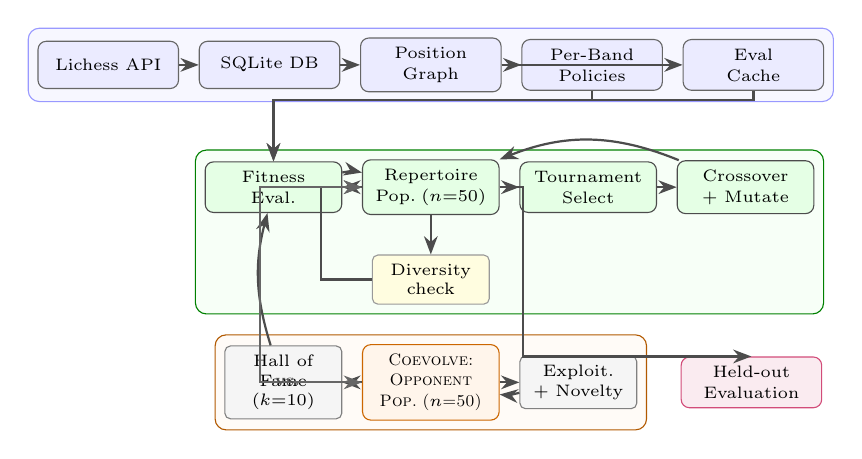
\begin{tikzpicture}[
    node distance=0.30cm and 0.25cm,
    box/.style={
      rectangle, rounded corners=3pt, draw=black!60,
      fill=blue!8, minimum height=0.60cm, text width=1.55cm,
      align=center, font=\fontsize{6.5}{7.5}\selectfont
    },
    gabox/.style={
      rectangle, rounded corners=3pt, draw=black!70,
      fill=green!10, minimum height=0.55cm, text width=1.50cm,
      align=center, font=\fontsize{6.5}{7.5}\selectfont
    },
    obox/.style={
      rectangle, rounded corners=3pt, draw=orange!80!black,
      fill=orange!8, minimum height=0.55cm, text width=1.50cm,
      align=center, font=\fontsize{6.5}{7.5}\selectfont
    },
    smallbox/.style={
      rectangle, rounded corners=2pt, draw=black!50,
      fill=gray!8, minimum height=0.50cm, text width=1.25cm,
      align=center, font=\fontsize{6}{7}\selectfont
    },
    arr/.style={-Stealth, thick, black!70},
    darr/.style={Stealth-Stealth, thick, black!60},
    label/.style={font=\fontsize{6}{7}\selectfont, text=black!70}
  ]

  % Row 1: Data pipeline
  \node[box] (api)    {Lichess API};
  \node[box, right=of api]  (db)    {SQLite DB};
  \node[box, right=of db]   (graph) {Position\\Graph};
  \node[box, right=of graph](pol)   {Per-Band\\Policies};
  \node[box, right=of pol]  (ec)    {Eval\\Cache};

  \draw[arr] (api) -- (db);
  \draw[arr] (db)  -- (graph);
  \draw[arr] (graph) -- (pol);
  \draw[arr] (graph) -- (ec);

  % Row 2: GA core (repop centred under graph)
  \node[gabox, below=0.85cm of graph] (repop) {Repertoire\\Pop.\;($n$=50)};
  \node[gabox, left=of repop]  (fit) {Fitness\\Eval.};
  \node[gabox, right=of repop] (sel) {Tournament\\Select};
  \node[gabox, right=of sel]   (cop) {Crossover\\+ Mutate};

  \draw[arr] (repop) -- (fit);
  \draw[arr] (fit)   edge[bend left=12] (repop);
  \draw[arr] (repop) -- (sel);
  \draw[arr] (sel)   -- (cop);
  \draw[arr] (cop)   edge[bend right=22] (repop);

  % Policies and cache feed fitness
  \draw[arr] (pol) -- ++(0,-0.45) -| (fit);
  \draw[arr] (ec)  -- ++(0,-0.45) -| (fit);

  % Diversity reinit — placed BELOW repop (avoids overlap with fit)
  \node[smallbox, below=0.50cm of repop, fill=yellow!12, draw=black!40]
    (div) {Diversity\\check};
  \draw[arr] (repop.south) -- (div.north);
  % reinit arc routes left of fit to return to repop
  \draw[arr] (div.west) -- ++(-0.65,0) |- (repop.west);

  % Row 3: Opponent co-evolution (COEVOLVE only) — below div
  \node[obox, below=0.50cm of div] (oppop) {\scshape Coevolve:\\Opponent\\Pop.\;($n$=50)};
  \node[smallbox, left=of oppop]  (hof) {Hall of\\Fame ($k$=10)};
  \node[smallbox, right=of oppop] (nov) {Exploit.\\+ Novelty};

  \draw[arr] (oppop) -- (hof);
  \draw[arr] (hof)   edge[bend left=16] (fit);
  \draw[arr] (oppop) -- (nov);
  \draw[arr] (nov)   edge[bend left=10] (oppop);

  % vs. arrow routes left of fit column to avoid div
  \draw[darr] (repop.west) -- ++(-1.30,0)
              |- node[label, right=2pt]{vs.} (oppop.west);

  % Held-out eval — right of nov, same height
  \node[box, right=0.55cm of nov, fill=purple!8, draw=purple!70]
    (heldout) {Held-out\\Evaluation};
  \draw[arr] (repop.east) -- ++(0.30,0) |- (heldout.north);

  % Bounding boxes + labels
  \begin{scope}[on background layer]
    \node[draw=blue!40, fill=blue!3, rounded corners=4pt,
          fit=(api)(db)(graph)(pol)(ec),
          label={[label, yshift=1pt]above:\textbf{Data Pipeline (C1--C4)}}] {};
    \node[draw=green!50!black, fill=green!3, rounded corners=4pt,
          fit=(repop)(fit)(sel)(cop)(div),
          label={[label]below:\textbf{GA Loop (C5--C8, 100 gens)}}] {};
    \node[draw=orange!70!black, fill=orange!3, rounded corners=4pt,
          fit=(oppop)(hof)(nov),
          label={[label]below:\textbf{Co-evolution ({\scshape Coevolve} only)}}] {};
  \end{scope}

  \end{tikzpicture}%
  }
  \caption{System architecture. The data pipeline (blue) crawls Lichess,
    builds a position graph, and precomputes per-band policies and empirical-Bayes
    evaluation scores. The GA loop (green) optimizes a population of repertoires
    via tournament selection, subtree-graft crossover, and four mutation operators,
    with diversity reinitialization when mean pairwise Jaccard distance falls
    below 0.25. {\scshape Coevolve} (orange) additionally maintains a co-evolving
    opponent population whose fitness balances exploitation and novelty, maintaining
    a Hall of Fame of the 10 most informative past opponents. Held-out evaluation
    (purple) uses a separate data split.}
  \label{fig:arch}
\end{figure}

Fig.~\ref{fig:arch} shows the overall system architecture. The pipeline
comprises two phases: data preprocessing (components C1--C4) and GA
optimization (C5--C8).

\subsection{Repertoire Chromosome and Initialization}

Each individual in the GA population is a \emph{candidate}: a paired
white and black repertoire sharing the same position graph and subject to
the same budget $B$. The initial population of $n = 50$ candidates is
seeded with a 50/50 mix of two strategies:
\begin{itemize}
  \item \textbf{Greedy initialization:} at each our-turn node, commit the
        move with the highest aggregate play frequency; expand opponent replies
        to closure.
  \item \textbf{Random initialization:} at each our-turn node, sample
        a move proportional to aggregate frequency; expand to closure.
\end{itemize}

\subsection{Mutation Operators}

Four mutation operators are applied with equal probability:
\begin{enumerate}
  \item \textbf{Move swap:} select a random committed node; replace its
        move with another legal move; rebuild the subtree below.
  \item \textbf{Extend:} select a random leaf (committed node with no
        further committed descendants); commit a new move and expand to
        closure if budget permits.
  \item \textbf{Prune:} select a random committed node; remove all
        committed moves in its subtree (reverts that branch to a leaf).
  \item \textbf{Opening replacement:} select a committed node at ply
        $\leq 5$; replace its move and reconstruct the subtree below
        via random initialization.
\end{enumerate}

Every mutation attempt enforces both the budget and closure constraints.
If a constraint cannot be satisfied, the attempt fails and is retried;
after 5 failed retries, the parent is returned unchanged.

\subsection{Crossover}

Crossover works by finding positions where both parents commit to the
\emph{same} move---these are shared pivot points. If any such pivots exist,
one is sampled at random, and the offspring inherits parent A's decisions
from the root down to the pivot and parent B's subtree below it. If the
combined result would exceed the budget, the operation fails and parent A
is returned unchanged. The same fallback applies when no shared pivot exists.
The crossover rate is $p_c = 1.0$.

\subsection{Selection and Diversity Maintenance}

We use tournament selection with size $k = 2$. To prevent the population
from collapsing to a single solution too quickly, we monitor mean pairwise
Jaccard distance over the committed move sets after each generation. If
this falls below $J_{\min} = 0.25$---meaning candidates have grown too
similar to one another---25\% of the population is replaced with freshly
random-initialized candidates.

\subsection{Co-evolutionary Opponent Model}

In {\scshape Coevolve}, the opponent is not fixed---it also evolves.
Each opponent is represented as a mixture $\boldsymbol{\pi} \in \Delta^2$
over the three rating bands, where $\Delta^2$ is the 3-simplex. Intuitively,
this encodes how much weight to give each skill level when evaluating a
repertoire. The {\scshape Coevolve} variant maintains 50 such opponent
chromosomes, each scored against the current repertoire population with:
\begin{equation}
  f_{\mathrm{opp}}(\boldsymbol{\pi}) =
  -\overline{F}(\boldsymbol{\pi}) + \eta \cdot d_{\text{nov}}(\boldsymbol{\pi}),
  \label{eq:oppfit}
\end{equation}
Here $\overline{F}(\boldsymbol{\pi})$ is the mean repertoire fitness under
mixture $\boldsymbol{\pi}$ (negated because a strong opponent is one that
produces low scores), $d_{\text{nov}}$ is the mean $\ell_2$ distance to all
other current opponents, and $\eta = 0.5$ is the novelty weight. Opponents
reproduce via convex-blend crossover ($p_c = 1.0$) and Dirichlet-noise
mutation, where the updated mixture is $\boldsymbol{\pi}' =
(1 - s)\,\boldsymbol{\pi} + s\,\mathbf{d}$ with
$\mathbf{d} \sim \mathrm{Dir}(\mathbf{1})$ and strength $s = 0.5$.

A key challenge in co-evolution is evaluation instability: because the
opponent population changes every generation, fitness scores are difficult
to compare across time. To address this, we maintain a \textbf{Hall of
Fame} of the 10 opponents with the highest fitness-variance across the
current repertoire population---in other words, the opponents that best
discriminate between strong and weak repertoires. Repertoire fitness is
evaluated against these Hall-of-Fame opponents rather than the current
opponent population, providing a stable evaluation signal across generations.

\subsection{Fitness Evaluation for Repertoires}

In {\scshape Static}, every repertoire is evaluated against a fixed uniform
mixture $\boldsymbol{\pi} = (1/3, 1/3, 1/3)$, treating all three rating
bands equally throughout training. In {\scshape Coevolve}, each repertoire
is instead scored against all current Hall-of-Fame opponents, and its
fitness is the mean across them. Per-band scores $s_b(\mathcal{R})$ are
cached on the candidate and reused when the same repertoire faces multiple
opponents in the same generation, avoiding redundant computation.

\subsection{Non-GA Baselines}

To give context for what the GA actually buys, we include three
non-evolutionary baselines, each given the same evaluation budget of
6,000 fitness evaluations:
\begin{itemize}
  \item \textbf{Most-played:} a single greedy pass from the root,
        always committing the most popular move; no search.
  \item \textbf{Random search:} sample 6,000 random candidates
        (via random initialization), return the best.
  \item \textbf{Greedy hillclimb:} start from the greedy solution;
        apply 6,000 random mutations, accepting each only if fitness
        improves ($= (1{+}1)$-ES).
\end{itemize}


% =========================================================================
\section{Experimental Setup}

\textbf{Data.} We use Lichess rapid and classical games crawled via
the Lichess Opening Explorer API. The training split covers all games
before June 2025; the held-out split covers games from June 2025 onwards.
The position graph includes all positions up to $D_{\max} = 10$ ply
(five full moves per side).

\textbf{Methods.} We evaluate five methods: \textsc{Baseline}
(most-played), \textsc{Random}, \textsc{Hillclimb}, \textsc{Static},
and \textsc{Coevolve}. To isolate the contribution of the closure rule,
we also run two ablation variants---\textsc{Static-NoClosure} and
\textsc{Coevolve-NoClosure}---that disable it entirely.

\textbf{Budget conditions.} All methods run under two budget constraints:
$B = 10$ committed moves per color (our primary condition) and $B = 25$
(secondary), representing compact and expanded repertoires respectively.

\textbf{Hyperparameters.} All fixed hyperparameters are listed in
Table~\ref{tab:hyperparams}.

\begin{table}[!t]
  \centering
  \caption{Fixed hyperparameters used in all experiments.}
  \label{tab:hyperparams}
  \renewcommand{\arraystretch}{1.10}
  \setlength{\tabcolsep}{5pt}
  \begin{tabular}{lc}
    \toprule
    \textbf{Parameter} & \textbf{Value} \\
    \midrule
    Repertoire population $n_R$   & 50 \\
    Opponent population $n_O$     & 50 \\
    Generations $G$               & 100 \\
    Tournament size $k$           & 2 \\
    Crossover rate $p_c$          & 1.0 \\
    Mutation rate $p_m$           & 0.5 \\
    Closure threshold $\theta$    & 0.15 \\
    CVaR weight $\lambda$         & 1.0 \\
    Novelty weight $\eta$         & 0.5 \\
    Hall of Fame size             & 10 \\
    Diversity threshold $J_{\min}$& 0.25 \\
    Policy smoothing $\alpha$     & 5.0 \\
    Score shrinkage $\tau$        & 20 \\
    Max ply depth $D_{\max}$      & 10 \\
    Seeds                         & 30 (1000--1029) \\
    \bottomrule
  \end{tabular}
\end{table}

\textbf{Seeds and reproducibility.} All methods run with the same 30
independent random seeds (1000--1029), enabling paired statistical tests
that control for run-to-run variability.

\textbf{Evaluation metrics.}
The primary metric is the \textbf{held-out uniform mean score}: the fitness
of the best candidate from each run, evaluated on held-out data under the
uniform opponent mixture. The secondary metric is the \textbf{held-out
worst-band score}: the minimum score across the three rating bands, which
serves as a proxy for robustness.

\textbf{Statistics.} We report mean $\pm$ standard deviation across 30
seeds. Pairwise comparisons use two-sided Wilcoxon signed-rank tests
(paired within seed) with Holm correction for multiple comparisons.
Effect sizes use the Vargha-Delaney $A_{12}$ statistic: $A_{12} < 0.5$
means method A is worse, $A_{12} > 0.5$ means method A is better, and
$A_{12} = 0.5$ indicates no difference.


% =========================================================================
\section{Results}

\subsection{Main Comparison}

The three optimized methods---Hillclimb, \textsc{Static}, and
\textsc{Coevolve}---converge to essentially the same held-out score, while
the most-played baseline and random search fall well behind. At $B = 10$,
all three reach $0.527 \pm 0.002$ against the baseline's $0.498$---a gap
of roughly 3 percentage points (Table~\ref{tab:main}). Random search scores
$0.522 \pm 0.002$, meaningfully lower than the other optimized methods
despite the same evaluation budget. The pattern repeats at $B = 25$, where
the optimized methods reach $0.525 \pm 0.002$ versus $0.492$ for the
baseline. One somewhat surprising result: $B = 10$ slightly outperforms
$B = 25$, suggesting that a tighter budget pushes the algorithm toward
higher-value lines.

\begin{table}[!t]
  \centering
  \caption{Held-out scores (mean $\pm$ std, $n=30$ seeds). \textit{Uniform
    mean}: expected score under uniform opponent mixture. \textit{Worst
    band}: minimum score across the three rating bands (CVaR proxy).
    Bold indicates the top tier (Hillclimb, \textsc{Static},
    \textsc{Coevolve} are statistically indistinguishable).}
  \label{tab:main}
  \renewcommand{\arraystretch}{1.15}
  \setlength{\tabcolsep}{3.5pt}
  \begin{tabular}{l cc cc}
    \toprule
    & \multicolumn{2}{c}{\textbf{Budget 10 (Primary)}}
    & \multicolumn{2}{c}{\textbf{Budget 25}} \\
    \cmidrule(lr){2-3}\cmidrule(lr){4-5}
    \textbf{Method} & \textit{Unif.~mean} & \textit{Worst~band}
                    & \textit{Unif.~mean} & \textit{Worst~band} \\
    \midrule
    Baseline        & $0.498 \pm 0.000$ & $0.493 \pm 0.000$
                    & $0.492 \pm 0.000$ & $0.488 \pm 0.000$ \\
    Random search   & $0.522 \pm 0.002$ & $0.515 \pm 0.001$
                    & $0.518 \pm 0.002$ & $0.513 \pm 0.001$ \\
    Hillclimb       & $\mathbf{0.527 \pm 0.003}$ & $\mathbf{0.521 \pm 0.002}$
                    & $\mathbf{0.525 \pm 0.002}$ & $\mathbf{0.520 \pm 0.001}$ \\
    \textsc{Static} & $\mathbf{0.527 \pm 0.002}$ & $\mathbf{0.521 \pm 0.002}$
                    & $\mathbf{0.525 \pm 0.002}$ & $\mathbf{0.520 \pm 0.002}$ \\
    \textsc{Coevolve} & $\mathbf{0.527 \pm 0.002}$ & $\mathbf{0.521 \pm 0.002}$
                      & $\mathbf{0.525 \pm 0.002}$ & $\mathbf{0.520 \pm 0.002}$ \\
    \bottomrule
  \end{tabular}
\end{table}

\begin{figure}[!t]
  \centering
  
\includegraphics[width=\columnwidth]{results_10/score_distributions.png}
  \caption{Distribution of held-out uniform mean scores across 30 seeds
    at $B = 10$. Box plots show median, IQR, and 1.5$\times$IQR whiskers;
    individual seed scores are overlaid. The three optimized methods
    (Hillclimb, \textsc{Static}, \textsc{Coevolve}) are
    statistically indistinguishable from each other ($p \geq 0.98$,
    Wilcoxon + Holm), while all significantly outperform Random and Baseline.}
  \label{fig:score_dist}
\end{figure}

Fig.~\ref{fig:score_dist} shows the full score distributions at $B = 10$.
The three optimized methods are statistically indistinguishable from one
another: Wilcoxon $p \geq 0.98$ and $A_{12} \in [0.45, 0.54]$ for all
pairwise comparisons (Table~\ref{tab:pairwise}). All three significantly
outperform random search ($p < 10^{-7}$, $A_{12} \leq 0.07$) and the
most-played baseline ($p < 1.5 \times 10^{-8}$, $A_{12} = 0.0$, meaning
no baseline seed beats any optimized seed).

\begin{table}[!t]
  \centering
  \caption{Pairwise comparison at $B = 10$ (held-out uniform mean score,
    $n=30$ paired seeds). $p$-values are Holm-corrected Wilcoxon. $A_{12}$:
    Vargha-Delaney effect size (row method vs.\ column method;
    $> 0.5$ means row is better).
    \cmark = significant at $\alpha = 0.05$.}
  \label{tab:pairwise}
  \renewcommand{\arraystretch}{1.12}
  \setlength{\tabcolsep}{3.5pt}
  \small
  \begin{tabular}{lcccc}
    \toprule
    \textbf{Method A vs.\ B} & \textbf{$\Delta$ mean} & \textbf{$p$-val} & \textbf{$A_{12}$} & \textbf{Sig.} \\
    \midrule
    Baseline vs.\ Random       & $-0.024$ & $<10^{-8}$ & 0.00 & \cmark \\
    Baseline vs.\ Hillclimb    & $-0.029$ & $<10^{-8}$ & 0.00 & \cmark \\
    Baseline vs.\ \textsc{Static}  & $-0.029$ & $<10^{-8}$ & 0.00 & \cmark \\
    Baseline vs.\ \textsc{Coevolve}& $-0.029$ & $<10^{-8}$ & 0.00 & \cmark \\
    Random vs.\ Hillclimb      & $-0.005$ & $<10^{-7}$ & 0.07 & \cmark \\
    Random vs.\ \textsc{Static}    & $-0.005$ & $<10^{-8}$ & 0.06 & \cmark \\
    Random vs.\ \textsc{Coevolve}  & $-0.005$ & $<10^{-8}$ & 0.03 & \cmark \\
    Hillclimb vs.\ \textsc{Static} & $+0.000$ & $1.00$      & 0.54 & -- \\
    Hillclimb vs.\ \textsc{Coevolve} & $-0.000$ & $0.98$    & 0.51 & -- \\
    \textsc{Static} vs.\ \textsc{Coevolve} & $-0.000$ & $1.00$ & 0.45 & -- \\
    \bottomrule
  \end{tabular}
\end{table}

\subsection{GA vs.\ Non-GA Baselines}

\begin{figure}[!t]
  \centering
  
\includegraphics[width=\columnwidth]{results_10/ga_vs_nonga.png}
  \caption{GA methods vs.\ non-GA baselines at $B = 10$.
    Per-seed scores are shown; methods sorted by mean within groups.
    Hillclimb reaches GA-level quality at ${\sim}1/35$ of
    {\scshape Coevolve}'s runtime.}
  \label{fig:ga_vs_nonga}
\end{figure}

The key takeaway from Fig.~\ref{fig:ga_vs_nonga} is that the greedy
hillclimber matches both GA methods in final quality, with tighter spread
at $B = 10$. It is not a sophisticated algorithm---just steepest-ascent
mutations from a greedy initialization---yet it finds solutions that neither
GA variant can improve upon. Random search, which samples 6,000 candidates
without structure, is significantly worse than all three, confirming that
directed local exploration pays off on this landscape.

\subsection{Closure Ablation}

\begin{figure}[!t]
  \centering
  
\includegraphics[width=\columnwidth]{results_10/closure_ablation.png}
  \caption{Closure ON vs.\ OFF at $B = 10$, for \textsc{Static} and
    \textsc{Coevolve}. Each point is one seed. Closure consistently
    improves every seed: $A_{12} = 1.0$ in all four comparisons.}
  \label{fig:closure}
\end{figure}

\begin{table}[!t]
  \centering
  \caption{Closure ablation results (held-out uniform mean and worst-band
    scores). $\Delta = $ score with closure $-$ score without.
    All comparisons: Wilcoxon $p < 7.5 \times 10^{-9}$, $A_{12} = 1.0$
    (perfect effect size, $n = 30$ paired seeds).}
  \label{tab:closure}
  \renewcommand{\arraystretch}{1.12}
  \setlength{\tabcolsep}{4pt}
  \begin{tabular}{llccc}
    \toprule
    \textbf{Metric} & \textbf{Method} & \textbf{With} & \textbf{Without} & \textbf{$\Delta$} \\
    \midrule
    \multirow{2}{*}{Unif.\ mean}
      & \textsc{Static}   & 0.5269 & 0.5037 & $+0.0232$ \\
      & \textsc{Coevolve} & 0.5272 & 0.5037 & $+0.0235$ \\
    \midrule
    \multirow{2}{*}{Worst band}
      & \textsc{Static}   & 0.5209 & 0.5023 & $+0.0187$ \\
      & \textsc{Coevolve} & 0.5211 & 0.5023 & $+0.0188$ \\
    \bottomrule
  \end{tabular}
\end{table}

The closure rule turns out to be the single most important component of
the system. Removing it drops mean score by 2.3~pp at $B = 10$ (2.15~pp
at $B = 25$), with $A_{12} = 1.0$: every one of the 30 seeds performs
worse without the rule, no exceptions (Table~\ref{tab:closure},
Fig.~\ref{fig:closure}). Worst-band score drops by 1.9~pp as well,
confirming that closure improves robustness, not just average performance.
The statistical evidence is unambiguous: Wilcoxon $p < 7.5 \times 10^{-9}$
with Holm correction. Notably, both \textsc{Static} and \textsc{Coevolve}
converge to the same no-closure score of $0.5037$, suggesting the
unconstrained landscape has a dominant basin that the GA locates quickly
regardless of variant.

\subsection{Robustness Across Rating Bands}

\begin{figure}[!t]
  \centering
  
\includegraphics[width=\columnwidth]{results_10/band_breakdown.png}
  \caption{Per-band scores at $B = 10$. The three rating bands show
    meaningfully different score profiles, confirming that optimizing
    for robustness across bands is non-trivial.}
  \label{fig:band}
\end{figure}

Fig.~\ref{fig:band} reveals why a mean-only objective would be
insufficient: the three rating bands show meaningfully different score
profiles, with gaps of several percentage points between them. A repertoire
that performs well against mid-range players does not automatically hold up
against beginners or advanced opponents. The CVaR term in the fitness
explicitly penalizes this variation. In practice, all optimized methods
achieve comparable per-band robustness, with worst-band scores tracking
the uniform mean closely (Table~\ref{tab:main}).

\subsection{GA Convergence Dynamics}

\begin{figure}[!t]
  \centering
  
\includegraphics[width=\columnwidth]{results_25/convergence.png}
  \caption{Training fitness over 100 generations at $B = 25$, across
    30 seeds (mean $\pm$ 95\% CI). \textsc{Coevolve} shows slightly
    higher initial variance due to opponent adaptation; all methods
    converge by approximately generation 30.}
  \label{fig:conv}
\end{figure}

Fig.~\ref{fig:conv} shows training fitness over 100 generations at
$B = 25$. Both {\scshape Static} and {\scshape Coevolve} improve rapidly
in the first 30 generations, then plateau. Their 95\% confidence intervals
overlap throughout the entire run---co-evolution provides neither a faster
trajectory nor a higher ceiling. The diversity reinitialization mechanism
keeps the population from converging prematurely; mean pairwise Jaccard
distance settles at roughly $0.35$--$0.40$ in later generations
(visible in Fig.~\ref{fig:dyn}).

\subsection{Coevolution Dynamics}

\begin{figure}[!t]
  \centering
  
\includegraphics[width=\columnwidth]{results_25/coevolve_dynamics.png}
  \caption{{\scshape Coevolve} population dynamics at $B = 25$ over
    100 generations (mean across 30 seeds). \emph{Top}: training
    fitness. \emph{Middle}: repertoire diversity (mean pairwise Jaccard).
    \emph{Bottom}: opponent diversity (mean pairwise $\ell_2$). The Hall
    of Fame reaches capacity ($k=10$) immediately and remains constant;
    opponent diversity stabilizes at ${\approx}0.28$ after ${\sim}10$ generations.}
  \label{fig:dyn}
\end{figure}

Fig.~\ref{fig:dyn} tracks three aspects of co-evolutionary behavior at
$B = 25$. Repertoire diversity begins high ($\approx 0.86$ mean pairwise
Jaccard) and settles around $0.35$ by generation 25, with occasional spikes
from diversity reinitialization. Opponent diversity stabilizes quickly at
$\approx 0.28$ after about 10 generations, showing that the opponent
population does maintain a spread of strategies. The Hall of Fame fills to
its full capacity of 10 opponents by generation 0 and stays there---diverse,
informative opponents are available from the very start. Yet despite all
this adaptive machinery, the repertoire fitness trajectory is
indistinguishable from {\scshape Static}, which explains the null result
in Table~\ref{tab:pairwise}.

\subsection{Example Repertoire}

\begin{figure}[!t]
  \centering
  
\includegraphics[width=\columnwidth]{results_25/repertoire_graph_COEVOLVE.png}
  \caption{Best {\scshape Coevolve} repertoire at $B = 25$ (seed 1008),
    visualized as a decision graph. Our-color committed moves are shown
    as filled nodes; opponent responses appear as branching edges.
    The repertoire covers major opening families including the Queen's
    Gambit, Gr\"unfeld Defense, Sicilian Defense, Benoni, and Caro-Kann.}
  \label{fig:repgraph}
\end{figure}

Fig.~\ref{fig:repgraph} shows a concrete example of what an optimized
repertoire looks like. The effect of the closure rule is visible in the
structure: at key decision points the tree branches to cover multiple
opponent continuations rather than committing to a single line. The
repertoire commits 21 moves as White and 24 as Black, nearly exhausting
the budget of 25, and spans major opening families including the Queen's
Gambit, Gr\"unfeld, Sicilian, Benoni, and Caro-Kann.

\subsection{Computational Cost}

\begin{table}[!t]
  \centering
  \caption{Wall-clock runtime (mean $\pm$ std, $n=30$ seeds).
    Evaluation budget: 6,000 fitness evaluations for all methods.}
  \label{tab:runtime}
  \renewcommand{\arraystretch}{1.12}
  \setlength{\tabcolsep}{4pt}
  \begin{tabular}{l cc}
    \toprule
    \textbf{Method} & \textbf{$B=10$ runtime (s)} & \textbf{$B=25$ runtime (s)} \\
    \midrule
    Baseline        & $0.03 \pm 0.01$  & $0.07 \pm 0.01$  \\
    Random search   & $2.85 \pm 0.11$  & $13.98 \pm 5.35$ \\
    Hillclimb       & $1.03 \pm 0.06$  & $5.16 \pm 1.35$  \\
    \textsc{Static} & $2.67 \pm 0.47$  & $33.97 \pm 129.1$\\
    \textsc{Coevolve} & $92.4 \pm 11.6$& $371.6 \pm 122.9$\\
    \bottomrule
  \end{tabular}
\end{table}

The runtime differences between methods are stark (Table~\ref{tab:runtime}).
{\scshape Coevolve} takes $35\times$ longer than {\scshape Static} at
$B = 10$ and $11\times$ longer at $B = 25$, yet produces no measurable
improvement in held-out score. The greedy hillclimber is the clear
efficiency winner, reaching {\scshape Static}-equivalent quality in just
$1.0$~s at $B = 10$.


% =========================================================================
\section{Discussion}

\textbf{The closure rule is the decisive contribution.}
The most important takeaway from this work is not the GA---it is the
closure rule. Removing it drops performance by 2.3~pp with perfect effect
size ($A_{12} = 1.0$), meaning every single seed across all 30 runs performs
worse without it. This holds for both GA variants and both budget conditions.
The closure rule enforces what we might call \emph{adversarial completeness}:
the repertoire must handle all likely opponent replies, not just the single
most popular continuation. Without this constraint, the GA exploits the
freedom to ignore inconvenient branches---producing repertoires that score
well on training data but would fail in practice as soon as the opponent
plays a common alternative.

\textbf{Co-evolution does not help.}
{\scshape Coevolve} was designed with principled co-evolutionary machinery:
adaptive opponent populations, novelty-driven fitness, and a Hall of Fame to
maintain evaluation stability. Yet it provides no statistically significant
benefit over {\scshape Static} ($p = 1.0$, $A_{12} = 0.45$). The most
likely explanation is that the opponent search space---a 3-simplex over three
rating bands---is simply too low-dimensional to offer meaningful adversarial
diversity. The uniform mixture already captures most of the signal, leaving
no useful gradient for co-evolution to exploit. A richer opponent model, such
as per-position move policies that vary by style rather than just rating,
might create enough adversarial pressure for co-evolution to pay off.

\textbf{Greedy hillclimbing is competitive.}
The greedy hillclimber matches both GA variants in final quality at roughly
$1/90$ of {\scshape Coevolve}'s cost at $B = 10$. This strongly suggests
that the closure-constrained fitness landscape is largely unimodal, or at
least contains a dominant basin of attraction that a simple local-search
procedure can reach. At the scales tested here, maintaining a population of
50 candidates brings no measurable benefit over a single trajectory of
steepest-ascent mutations.

\textbf{Budget 10 vs.\ Budget 25.}
The smaller budget slightly outperforms the larger one (0.5272 vs.\ 0.5252
for {\scshape Coevolve}), which at first seems counter-intuitive. One
explanation is that a tighter budget forces the algorithm to commit only to
the highest-value moves, while a larger budget allows it to fill remaining
space with marginal lines that dilute overall quality. Another possibility
is that $B = 25$ evaluations are individually more expensive, so 100
generations may not be enough for full convergence at the larger budget.

\textbf{Limitations.} The position graph covers only 10 ply, while real
games regularly branch deeper. The opponent model aggregates all players
within a rating band into a single mixture, ignoring individual style.
The evaluation metric---an empirical-Bayes win rate from historical
games---may not perfectly capture the value of a move when an opponent
knows they are facing a prepared repertoire. Addressing these gaps with
deeper crawls, individualized opponent models, and online evaluation against
real players would be natural next steps.


% =========================================================================
\section{Conclusion}

We have presented a system for automatically constructing robust chess
opening repertoires under a memorization budget constraint, combining a
genetic algorithm with a novel closure rule evaluated on real Lichess game
data. The central finding is that the closure rule---which requires the
repertoire to cover all opponent replies played in at least 15\% of observed
games---accounts for the bulk of the improvement. It yields a
+2.3~percentage-point gain in held-out expected score with perfect effect
size ($A_{12} = 1.0$, $p < 7.5 \times 10^{-9}$) across all 30 seeds and
both budget conditions. Without it, the GA exploits gaps in opponent coverage
to inflate training scores while undermining practical robustness.

The co-evolutionary component, despite its principled design, adds no
measurable benefit over a static GA ($p = 1.0$, $A_{12} = 0.45$) at
35$\times$ the computational cost. The likely cause is that the opponent
search space---three rating-band weights on a simplex---is too restricted
to generate meaningful adversarial pressure. More strikingly, a greedy
hillclimber matches GA-level quality at roughly 1/90 of {\scshape Coevolve}'s
runtime, suggesting the closure-constrained fitness landscape is well-suited
to simple local search.

Future work should explore deeper position graphs, more expressive opponent
models (e.g., per-position move policies that capture individual playing
style), and online adaptation based on real-game outcomes. The closure rule
concept may also generalize beyond chess to other adversarial preparation
problems where coverage completeness is essential---any domain where ignoring
a branch is a practical failure mode.

% =========================================================================
\section*{Acknowledgment}

This work was completed as part of the Computational Intelligence
(CS~462) course, Spring 2026, Habib University, Karachi, Pakistan.
Opening data is sourced from the Lichess Opening Explorer API under
the Creative Commons Attribution 4.0 license.

% =========================================================================
\begin{thebibliography}{9}

\bibitem{rosin1997}
    C.~D. Rosin and R.~K. Belew, ``New methods for competitive coevolution,''
    \textit{Evolutionary Computation}, vol.~5, no.~1, pp.~1--29, 1997.

\bibitem{fogel2004}
    D.~B. Fogel, ``A self-learning evolutionary chess program,''
    \textit{Proc. IEEE}, vol.~92, no.~12, pp.~1947--1964, Dec. 2004.

\bibitem{ramos2016}
    N.~Ramos, S.~Salgado, and A.~C. Rosa, ``Chess player by co-evolutionary
    algorithm,'' arXiv preprint arXiv:1605.06710, May 2016.

\bibitem{hillis1990}
    W.~D. Hillis, ``Co-evolving parasites improve simulated evolution as an
    optimization procedure,'' \textit{Physica D: Nonlinear Phenomena},
    vol.~42, no.~1--3, pp.~228--234, 1990.

\bibitem{walczak1996}
    S.~Walczak, ``Improving opening book performance through modeling of chess
    opponents,'' in \textit{Proc. ACM 24th Annu. Conf. Computer Science
    (CSC'96)}, Philadelphia, PA, USA, Feb. 1996, pp.~53--57.

\bibitem{marzo2023}
    G.~De Marzo and V.~D.~P. Servedio, ``Quantifying the complexity and
    similarity of chess openings using online chess community data,''
    \textit{Scientific Reports}, vol.~13, no.~1, p.~5327, Apr. 2023.

\bibitem{lehman2011}
    J.~Lehman and K.~O. Stanley, ``Abandoning objectives: Evolution through
    the search for novelty alone,'' \textit{Evolutionary Computation},
    vol.~19, no.~2, pp.~189--223, 2011.

\bibitem{rockafellar2000}
    R.~T. Rockafellar and S.~Uryasev, ``Optimization of conditional
    value-at-risk,'' \textit{Journal of Risk}, vol.~2, no.~3, pp.~21--41,
    2000.

\bibitem{lichess}
    Lichess.org, ``Lichess Opening Explorer API,'' 2025. [Online]. Available:
    \url{https://lichess.org/api}

\end{thebibliography}

\end{document}
